\documentclass[tikz,border=2mm]{standalone}
\usepackage{amsmath,amssymb}
\usetikzlibrary{arrows.meta,calc}
\newcommand{\tikzsetnextfilename}[1]{}

\definecolor{iconblue}{RGB}{70,140,255}

\tikzset{
  poset edge/.style={line width=0.8pt},
  poset node/.style={
    circle,
    draw=black,
    fill=white,
    line width=0.8pt,
    minimum size=8mm,
    inner sep=0pt
  },
  chosen/.style={fill=iconblue!65},
  action/.style={-{Stealth[length=2.2mm]},line width=0.9pt,draw=iconblue}
}

\newcommand{\labeledtwobythree}[8]{%
  \begin{scope}[xshift=#1,yshift=#2]
    \coordinate (a) at (0,0);
    \coordinate (b) at (-0.42,0.62);
    \coordinate (c) at (-0.84,1.24);
    \coordinate (d) at (0.42,0.62);
    \coordinate (e) at (0,1.24);
    \coordinate (f) at (-0.42,1.86);
    \draw[poset edge]
      (a) -- (b) -- (c) -- (f)
      (a) -- (d) -- (e) -- (f)
      (b) -- (e);
    \node[poset node,minimum size=5.4mm] at (a) {#3};
    \node[poset node,minimum size=5.4mm] at (b) {#4};
    \node[poset node,minimum size=5.4mm] at (c) {#5};
    \node[poset node,minimum size=5.4mm] at (d) {#6};
    \node[poset node,minimum size=5.4mm] at (e) {#7};
    \node[poset node,minimum size=5.4mm] at (f) {#8};
  \end{scope}%
}

\newcommand{\idealtwobythree}[8]{%
  \begin{scope}[xshift=#1,yshift=#2]
    \coordinate (a) at (0,0);
    \coordinate (b) at (-0.25,0.36);
    \coordinate (c) at (-0.50,0.72);
    \coordinate (d) at (0.25,0.36);
    \coordinate (e) at (0,0.72);
    \coordinate (f) at (-0.25,1.08);
    \draw[poset edge]
      (a) -- (b) -- (c) -- (f)
      (a) -- (d) -- (e) -- (f)
      (b) -- (e);
    \node[poset node,minimum size=4mm,font=\tiny,#3] at (a) {$a$};
    \node[poset node,minimum size=4mm,font=\tiny,#4] at (b) {$b$};
    \node[poset node,minimum size=4mm,font=\tiny,#5] at (c) {$c$};
    \node[poset node,minimum size=4mm,font=\tiny,#6] at (d) {$d$};
    \node[poset node,minimum size=4mm,font=\tiny,#7] at (e) {$e$};
    \node[poset node,minimum size=4mm,font=\tiny,#8] at (f) {$f$};
  \end{scope}%
}

\begin{document}

\tikzsetnextfilename{rowmotion-promotion-linear-extensions}
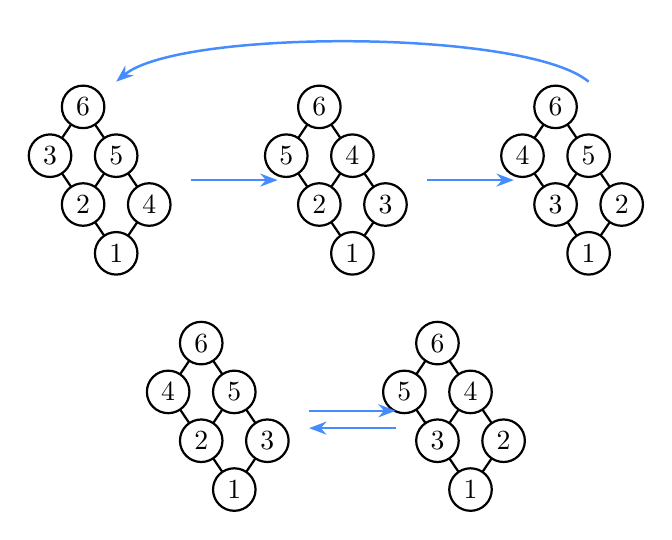
\begin{tikzpicture}
  \labeledtwobythree{0cm}{0cm}{1}{2}{3}{4}{5}{6}
  \labeledtwobythree{3cm}{0cm}{1}{2}{5}{3}{4}{6}
  \labeledtwobythree{6cm}{0cm}{1}{3}{4}{2}{5}{6}
  \draw[action] (0.95,0.93) -- (2.05,0.93);
  \draw[action] (3.95,0.93) -- (5.05,0.93);
  \draw[action]
    (6,2.18) .. controls (5.2,2.85) and (0.8,2.85) .. (0,2.18);

  \labeledtwobythree{1.5cm}{-3cm}{1}{2}{4}{3}{5}{6}
  \labeledtwobythree{4.5cm}{-3cm}{1}{3}{5}{2}{4}{6}
  \draw[action] (2.45,-2.00) -- (3.55,-2.00);
  \draw[action] (3.55,-2.22) -- (2.45,-2.22);
\end{tikzpicture}

\tikzsetnextfilename{rowmotion-promotion-order-ideals}
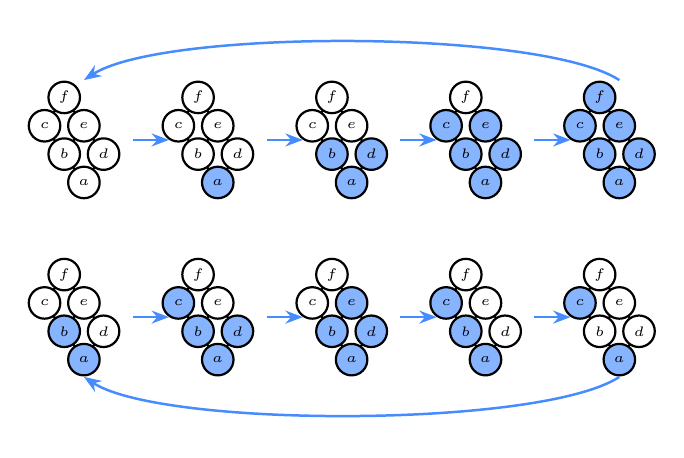
\begin{tikzpicture}
  \idealtwobythree{0cm}{0cm}{}{}{}{}{}{}
  \idealtwobythree{1.7cm}{0cm}{chosen}{}{}{}{}{}
  \idealtwobythree{3.4cm}{0cm}{chosen}{chosen}{}{chosen}{}{}
  \idealtwobythree{5.1cm}{0cm}{chosen}{chosen}{chosen}{chosen}{chosen}{}
  \idealtwobythree{6.8cm}{0cm}{chosen}{chosen}{chosen}{chosen}{chosen}{chosen}
  \foreach \x in {0,1.7,3.4,5.1} {
    \draw[action] ({\x+0.62},0.54) -- ({\x+1.08},0.54);
  }
  \draw[action]
    (6.8,1.30) .. controls (5.8,1.95) and (1.0,1.95) .. (0,1.30);

  \idealtwobythree{0cm}{-2.25cm}{chosen}{chosen}{}{}{}{}
  \idealtwobythree{1.7cm}{-2.25cm}{chosen}{chosen}{chosen}{chosen}{}{}
  \idealtwobythree{3.4cm}{-2.25cm}{chosen}{chosen}{}{chosen}{chosen}{}
  \idealtwobythree{5.1cm}{-2.25cm}{chosen}{chosen}{chosen}{}{}{}
  \idealtwobythree{6.8cm}{-2.25cm}{chosen}{}{chosen}{}{}{}
  \foreach \x in {0,1.7,3.4,5.1} {
    \draw[action] ({\x+0.62},-1.71) -- ({\x+1.08},-1.71);
  }
  \draw[action]
    (6.8,-2.47) .. controls (5.8,-3.12) and (1.0,-3.12) .. (0,-2.47);

\end{tikzpicture}

\end{document}
